\documentclass[landscape,paperheight=90cm,paperwidth=90cm,final]{baposter}
%below s added
%\documentclass[final, 12pt]{beamer}
%\documentclass[a4shrink,portrait,final]{baposter}
% Usa a4shrink for an a4 sized paper.

%\tracingstats=2

\usepackage{epsfig}
\usepackage{times}
\usepackage{calc}
\usepackage{graphicx}
\usepackage{amsmath}
\usepackage{amssymb}
\usepackage{relsize}
\usepackage{multirow}
\usepackage{bm}
\usepackage{enumitem}
\usepackage{multicol}
\usepackage{relsize,url}
\usepackage{graphics}
%below is added
%\usepackage[size=custom,orientation=portrait,scale=1.4,width =90, height=90,debug]{beamerposter}
\usepackage{pgfbaselayers}
\pgfdeclarelayer{background}
\pgfdeclarelayer{foreground}
\pgfsetlayers{background,main,foreground}

\usepackage{helvet}
\usepackage{bookman}
%\usepackage{palatino}
\usepackage{array}
\newcolumntype{L}[1]{>{\raggedright\let\newline\\\arraybackslash\hspace{0pt}}m{#1}}
\newcolumntype{C}[1]{>{\centering\let\newline\\\arraybackslash\hspace{0pt}}m{#1}}
\newcolumntype{R}[1]{>{\raggedleft\let\newline\\\arraybackslash\hspace{0pt}}m{#1}}
% mine

\usepackage{arydshln}
\usepackage{xspace,url,relsize}
\usepackage{mdwlist}

\newcommand{\corpus}[1]{\textsc{#1}\xspace}
\newcommand{\tool}[1]{\texttt{#1}\xspace}
\newcommand{\model}[1]{\textsc{#1}\xspace}

\newcommand{\topic}[1]{$\langle$\it#1$\rangle$}
\newcommand{\topiclabel}[1]{\textsc{#1}\xspace}
\newcommand{\dataset}[1]{\textsc{#1}\xspace}
\newcommand{\books}{\dataset{Books}}
\newcommand{\news}{\dataset{News}}
\newcommand{\blogs}{\dataset{Blogs}}
\newcommand{\pubmed}{\dataset{PubMed}}

\newcommand{\mymethod}[1]{\textsc{#1}\xspace}
\newcommand{\RACO}{\mymethod{raco}}

\newcounter{featcounter}
\newenvironment{featlist}{\begin{list}{\arabic{featcounter}.}{\usecounter{featcounter}}}{\end{list}}


\newsavebox{\fmbox}
\newenvironment{fmpage}[1]
{\begin{lrbox}{\fmbox}\begin{minipage}{#1}}
{\end{minipage}\end{lrbox}\fbox{\usebox{\fmbox}}}
% end mine

%\newcommand{\captionfont}{\footnotesize}

\selectcolormodel{cmyk}

\graphicspath{{img/}}

%%%%%%%%%%%%%%%%%%%%%%%%%%%%%%%%%%%%%%%%%%%%%%%%%%%%%%%%%%%%%%%%%%%%%%%%%%%%%%%%
%%%% Some math symbols used in the text
%%%%%%%%%%%%%%%%%%%%%%%%%%%%%%%%%%%%%%%%%%%%%%%%%%%%%%%%%%%%%%%%%%%%%%%%%%%%%%%%
% Format 
\newcommand{\Matrix}[1]{\begin{bmatrix} #1 \end{bmatrix}}
\newcommand{\Vector}[1]{\Matrix{#1}}
\newcommand*{\SET}[1]  {\ensuremath{\mathcal{#1}}}
\newcommand*{\MAT}[1]  {\ensuremath{\mathbf{#1}}}
\newcommand*{\VEC}[1]  {\ensuremath{\bm{#1}}}
\newcommand*{\CONST}[1]{\ensuremath{\mathit{#1}}}
\newcommand*{\norm}[1]{\mathopen\| #1 \mathclose\|}% use instead of $\|x\|$
\newcommand*{\abs}[1]{\mathopen| #1 \mathclose|}% use instead of $\|x\|$
\newcommand*{\absLR}[1]{\left| #1 \right|}% use instead of $\|x\|$
\newcommand{\spadeaff}{\ensuremath{\spadesuit}\xspace}
\newcommand{\clubaff}{\ensuremath{\clubsuit}\xspace}
\newcommand{\heartaff}{\ensuremath{\heartsuit}\xspace}
\newcommand{\diamondaff}{\ensuremath{\diamondsuit}\xspace}

\def\norm#1{\mathopen\| #1 \mathclose\|}% use instead of $\|x\|$
\newcommand{\normLR}[1]{\left\| #1 \right\|}% use instead of $\|x\|$

%%%%%%%%%%%%%%%%%%%%%%%%%%%%%%%%%%%%%%%%%%%%%%%%%%%%%%%%%%%%%%%%%%%%%%%%%%%%%%%%
% Multicol Settings
%%%%%%%%%%%%%%%%%%%%%%%%%%%%%%%%%%%%%%%%%%%%%%%%%%%%%%%%%%%%%%%%%%%%%%%%%%%%%%%%
\setlength{\columnsep}{0.7em}
\setlength{\columnseprule}{0mm}


%%%%%%%%%%%%%%%%%%%%%%%%%%%%%%%%%%%%%%%%%%%%%%%%%%%%%%%%%%%%%%%%%%%%%%%%%%%%%%%%
% Save space in lists. Use this after the opening of the list
%%%%%%%%%%%%%%%%%%%%%%%%%%%%%%%%%%%%%%%%%%%%%%%%%%%%%%%%%%%%%%%%%%%%%%%%%%%%%%%%
\newcommand{\compresslist}{%
\setlength{\itemsep}{0.2ex}%
\setlength{\parskip}{0.2ex}%
\setlength{\parsep}{0pt}%
}


%%%%%%%%%%%%%%%%%%%%%%%%%%%%%%%%%%%%%%%%%%%%%%%%%%%%%%%%%%%%%%%%%%%%%%%%%%%%%%
%%% Begin of Document
%%%%%%%%%%%%%%%%%%%%%%%%%%%%%%%%%%%%%%%%%%%%%%%%%%%%%%%%%%%%%%%%%%%%%%%%%%%%%%

\begin{document}

\larger
\sffamily

%%%%%%%%%%%%%%%%%%%%%%%%%%%%%%%%%%%%%%%%%%%%%%%%%%%%%%%%%%%%%%%%%%%%%%%%%%%%%%
%%% Here starts the poster
%%%---------------------------------------------------------------------------
%%% Format it to your taste with the options
%%%%%%%%%%%%%%%%%%%%%%%%%%%%%%%%%%%%%%%%%%%%%%%%%%%%%%%%%%%%%%%%%%%%%%%%%%%%%%
% Define some colors
\definecolor{silver}{cmyk}{0,0,0,0.3}
\definecolor{yellow}{cmyk}{0,0,0.9,0.0}
\definecolor{reddishyellow}{cmyk}{0,0.22,1.0,0.0}
\definecolor{black}{cmyk}{0,0,0.0,1.0}
\definecolor{darkYellow}{cmyk}{0,0,1.0,0.5}
\definecolor{darkSilver}{cmyk}{0,0,0,0.1}

\definecolor{darkGreen}{cmyk}{0.88,0,0.88,0.41}
\definecolor{midGreen}{cmyk}{0.71,0,0.66,0.01}

\definecolor{midBlue}{cmyk}{0.44,0.14,0,0.03}
\definecolor{lightSkyBlue}{cmyk}{0.31,0.11,0,0.00}
\definecolor{darkSkyBlue}{cmyk}{0.47,0.19,0,0.45}

\definecolor{darkRed}{cmyk}{0,1,1,0.56}
\definecolor{lightRed}{cmyk}{0,0.45,0.45,0.05}

\definecolor{myBlue}{rgb}{0.3,0.5,0.8}

%%
\typeout{Poster Starts}
\background{
  \begin{tikzpicture}[remember picture,overlay]%
    \draw (current page.north west)+(-2em,2em) node[anchor=north west] {\includegraphics[height=1.1\textheight]{silhouettes_background}};
  \end{tikzpicture}%
}

\newlength{\leftimgwidth}
\begin{poster}%
  % Poster Options
  {
  % Show grid to help with alignment
  grid=no,
  % Column spacing
  colspacing=0.8em,
  columns=4,
  % Color style
  bgColorOne=white,
  bgColorTwo=white,
  borderColor=darkSkyBlue,
  %borderColor=silver,
  %headerColorOne=midBlue,
  headerColorOne=myBlue,
  headerColorTwo=reddishyellow,
  headerFontColor=black,
  boxColorOne=white,
  boxColorTwo=white,
  % Format of textbox
  textborder=rounded,
  % Format of text header
  eyecatcher=no,
  headerborder=open,
  headerheight=0.17\textheight,
  headershape=rounded,
  headershade=plain,
  %headerfont=\Large\textsf, %Sans Serif
  headerfont=\Large\textsc, %Sans Serif
%  textfont=\sf,
  boxshade=plain,
%  background=shade-tb,
  background=plain,
  linewidth=1pt
  }
  % Eye Catcher

  {
  }
  % Title
  %{\sf\LARGE\vspace*{2em}
  {
\begin{tabular}{ccR{0.2cm}}
&  \bfseries Leveraging distributed representations and lexico-syntactic fixedness & \\
&  \multirow{3}{*\bfseries for token-level prediction of the idiomaticity of English verb-noun combinations }&\\
&\\
 & \textbf{Milton King and Paul Cook}  & \\
 & \smaller University of New Brunswick & \\
\end{tabular}
 
    \vspace*{3ex}

  }
  % Authors

  {}

%  \tikzstyle{light shaded}=[top color=baposterBGtwo!30!white,bottom 
%  color=baposterBGone!30!white,shading=axis,shading angle=30]
%
%  % Width of left inset image
%     \setlength{\leftimgwidth}{0.78em+8.0em}
%    % A coloured circle useful as a bullet with an adjustably strong filling
%    \newcommand{\colouredcircle}[1]{%
%      \tikz{\useasboundingbox (-0.2em,-0.32em) rectangle(0.2em,0.32em); \draw[draw=black,fill=baposterBGone!80!black!#1!white,line width=0.03em] (0,0) circle(0.18em);}}
%

%\begin{minipage}[b]{0.01\linewidth}
   %
\includegraphics[scale=0.083]{unbLogo.png}
   % \end{minipage}



%%%%%%%%%%%%%%%%%%%%%%%%%%%%%%%%%%%%%%%%%%%%%%%%%%%%%%%%%%%%%%%%%%%%%%%%%%%%%%
  \headerbox{Idiom Token Classification
}{name=usim,column=0,row=0,span=2}{
%%%%%%%%%%%%%%%%%%%%%%%%%%%%%%%%%%%%%%%%%%%%%%%%%%%%%%%%%%%%%%%%%%%%%%%%%%%%%%
\begin{itemize}
    \item Verb-noun combination (VNC): Multiword expression consisting of a verb and a noun.
    \item Task: Determine if an instance of a verb-noun combination is idiomatic.
\vspace{5mm}
\end{itemize}
\begin{tabular}{ll}
 \multirow{2}{*}{Idiomatic} & Hereford United were \underline{seeing stars} at Gillingham \\
&after letting in 2 early goals\\
\\
Literal &Look into the night sky to \underline{see} the
  \underline{stars} \\ 

\end{tabular}

}

%%%%%%%%%%%%%%%%%%%%%%%%%%%%%%%%%%%%%%%%%%%%%%%%%%%%%%%%%%%%%%%%%%%%%%%%%%%%%%
  \headerbox{Models
}{name=model,column=0,row=0,span=2, below=usim}{
%%%%%%%%%%%%%%%%%%%%%%%%%%%%%%%%%%%%%%%%%%%%%%%%%%%%%%%%%%%%%%%%%%%%%%%%%%%%%%
    \begin{itemize}
    %\item \textbf{Word embeddings:} Vector representations of words. Trained using the neural network based model. %%Do I have to cite? \citep{Mikolov+:2013a}
\item Considered three approaches to representing VNC instances as a vector.
\begin{itemize}
\item \textbf{1) Word2vec:} Average word2vec skipgram embeddings for the words in a sentence.
\item \textbf{2) Siamese CBOW:} Average siamese CBOW embeddings for the words in a sentence. 
\item \textbf{3) Skip-thoughts:} Autoencoder that is trained to generate an embedding for a sentence using recurrent neural networks.
\vspace{5mm}
\end{itemize}
\item \textbf{Supervised Model:} We trained an SVM for each of these representations. 

\end{itemize}

}

%%%%%%%%%%%%%%%%%%%%%%%%%%%%%%%%%%%%%%%%%%%%%%%%%%%%%%%%%%%%%%%%%%%%%%%%%%%%%%
  \headerbox{Dataset
}{name=mwe,column=0,row=0,span=2, below=model}{
%%%%%%%%%%%%%%%%%%%%%%%%%%%%%%%%%%%%%%%%%%%%%%%%%%%%%%%%%%%%%%%%%%%%%%%%%%%%%%
{\large
\setlength\extrarowheight{5pt}
        \begin{tabular}{l|cc|cc}
\multirow{2}{*}{}  &  \multicolumn{2}{c|}{DEV}  &  \multicolumn{2}{c}{TEST}\\
\cline{2-5}
& Training & Testing & Training & Testing\\
\hline
MWE types & 14 & 14 & 14 & 14\\
Idiom instances & 270& 92 &298 & 90\\
Literal instances& 179 & 53 & 172 & 53\\

\end{tabular}\\
	}


}



%Make biggger table
%%%%%%%%%%%%%%%%%%%%%%%%%%%%%%%%%%%%%%%%%%%%%%%%%%%%%%%%%%%%%%%%%%%%%%%%%%%%%%
  \headerbox{Canonical Forms
}{name=eval,column=2,row=0,span=2}{
%%%%%%%%%%%%%%%%%%%%%%%%%%%%%%%%%%%%%%%%%%%%%%%%%%%%%%%%%%%%%%%%%%%%%%%%%%%%%%

%%    Lexico-syntactic patterns describing VNC instances.\\ 
%% \\
%% \phantom{**} 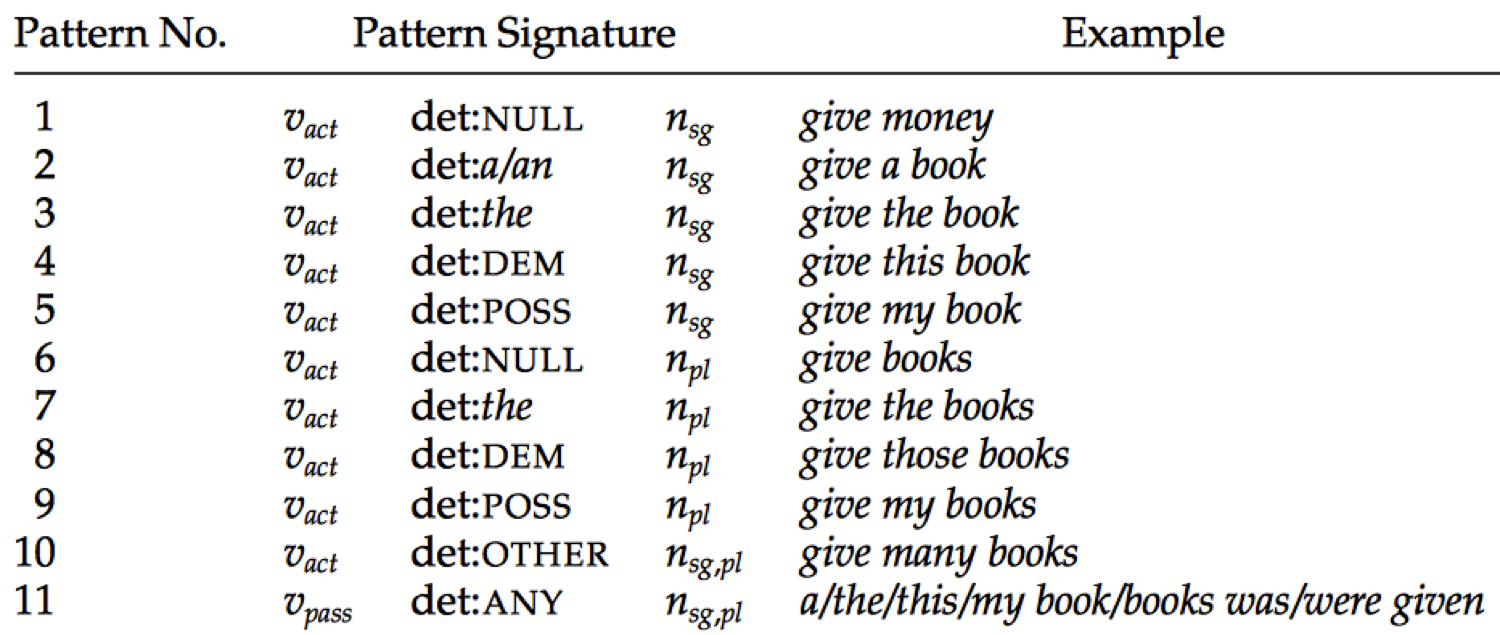
\includegraphics[scale=0.4]{conForms.png}\\

%% Idiomatic VNC usages tend to occur in 1 canonical form.
%% \vspace{3mm}

\begin{itemize}
\item   Lexico-syntactic patterns describing VNC instances.

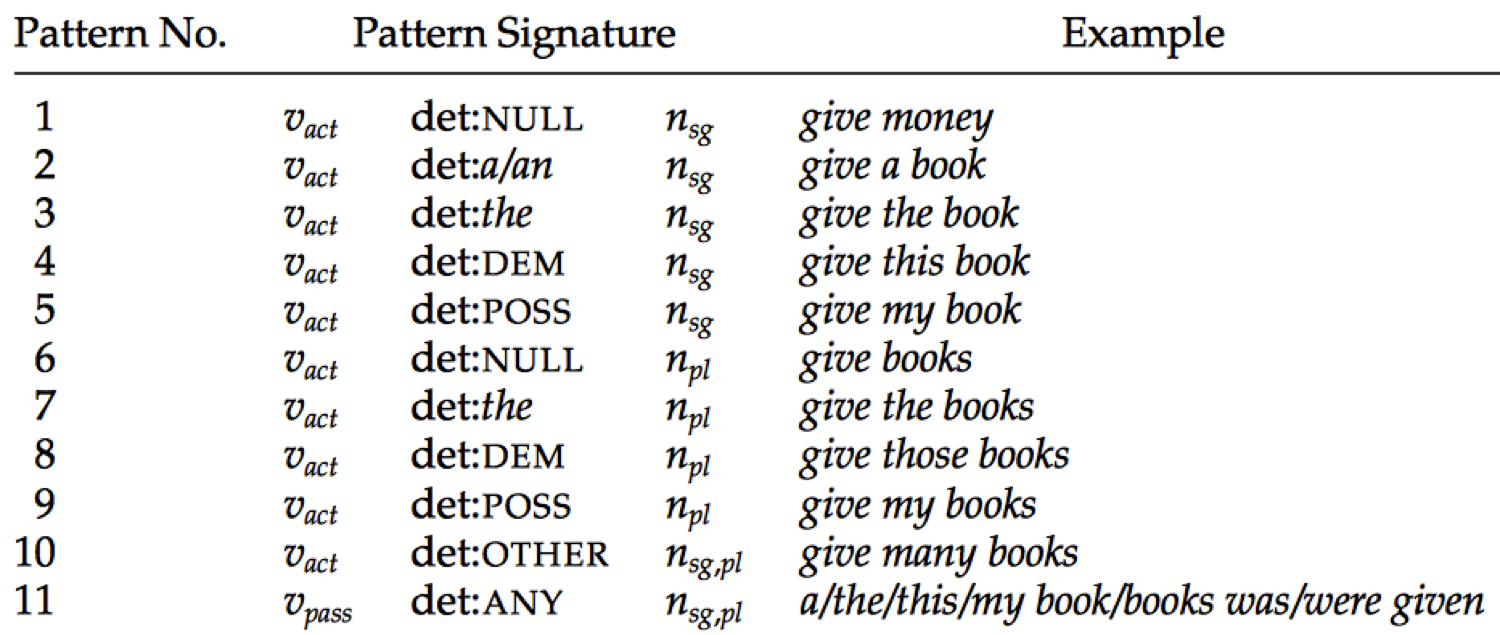
\includegraphics[scale=0.4]{conForms.png}

\item Idiomatic VNC usages tend to occur in 1 canonical form.
\end{itemize}
}




%%%%%%%%%%%%%%%%%%%%%%%%%%%%%%%%%%%%%%%%%%%%%%%%%%%%%%%%%%%%%%%%%%%%%%%%%%%%%%
  \headerbox{Results
}{name=results,column=2,row=0,span=2, below=eval}{
%%%%%%%%%%%%%%%%%%%%%%%%%%%%%%%%%%%%%%%%%%%%%%%%%%%%%%%%%%%%%%%%%%%%%%%%%%%%%%
 \begin{center}
{\large
\setlength\extrarowheight{5pt}
        \begin{tabular}{l|cc|cc}
\multirow{2}{*}{Model}  &  \multicolumn{2}{c|}{DEV}  &  \multicolumn{2}{c}{TEST}\\
\cline{2-5}
& $-$CF & $+$CF & $-$CF & $+$CF\\
\hline
CForm & - & 0.721 & - & 0.749\\
Word2vec &\textbf{0.830} &\textbf{0.854}& \textbf{0.804} &\textbf{0.852}\\
Siamese CBOW &0.763 &0.774 & 0.717 &0.779\\
Skip-thoughts &0.803 &0.827& 0.786 &0.842\\
%FastText &0.7381 &0.7445\\
%CNN-random &0.7799 &0.7557\\
%CNN-word2vec &0.8109 & -\\
\end{tabular}\\
	}



    \end{center}
}





%%%%%%%%%%%%%%%%%%%%%%%%%%%%%%%%%%%%%%%%%%%%%%%%%%%%%%%%%%%%%%%%%%%%%%%%%%%%%%
  \headerbox{Conclusions and Future Work
}{name=conclusion,column=2,row=0,span=2,below=results,bottomaligned=mwe}{
%%%%%%%%%%%%%%%%%%%%%%%%%%%%%%%%%%%%%%%%%%%%%%%%%%%%%%%%%%%%%%%%%%%%%%%%%%%%%%
    \begin{itemize}
    \item \textbf{Conclusions:}
\setlength{\itemindent}{+.2in}
\item Averaging word2vec embeddings outperforms the previously applied skip-thoughts model.
\item Employing information about canonical forms consistently improves all models.
\vspace{3mm}
\setlength{\itemindent}{0in}
    \item \textbf{Future Work:} Evaluate a word2vec model that is trained on the the same data as skip-thoughts.
\vspace{5mm}
%%Did not discuss per lemma
    \end{itemize}

}




\end{poster}%
\end{document}


%%% Local Variables: 
%%% mode: latex
%%% TeX-command-default: "Make"
%%% TeX-master: t
%%% End: 
